\documentclass[24pt, a4paper, oneside, spanish]{beamer}
\usetheme{Warsaw}

%Codificación e idioma
\usepackage[T1]{fontenc}
\usepackage[utf8]{inputenc}
\usepackage[spanish]{babel}

% Url
\usepackage{url}

% Graphics
%\usepackage[pdftex]{graphicx}
%\DeclareGraphicsExtensions{.png,.jpg}

\usepackage{wrapfig}

%Resaltado de sintaxis
\usepackage{color}
\definecolor{gray97}{gray}{.97}
\definecolor{gray75}{gray}{.75}
\definecolor{gray45}{gray}{.45}

\definecolor{red}{rgb}{0.6,0,0} % strings
\definecolor{green}{rgb}{0.25,0.5,0.35} % comments
\definecolor{purple}{rgb}{0.5,0,0.35} % keywords
\definecolor{blue}{rgb}{0.25,0.35,0.75} % doc

\usepackage{listings}
\lstset {
	language			= java,
	frame				=	Ltb,
    framerule			=	0pt,
    aboveskip			=	0.5cm,
    framextopmargin		=	3pt,
    framexbottommargin	=	3pt,
    framexleftmargin	=	0.4cm,
    framesep			=	0pt,
    rulesep				=	.4pt,
    backgroundcolor		=	\color{gray97},
    rulesepcolor		=	\color{black},
    %
    stringstyle			=	\color{red},
    showstringspaces	=	false,
    basicstyle			=	\ttfamily\small,
    commentstyle		=	\color{green},
    morecomment         =   [s][\color{blue}]{/*}{*/},
    keywordstyle		=	\color{purple}\bfseries,
    tabsize					=	3,
    %
    numbers				=	left,
    numbersep			=	15pt,
    numberstyle			=	\tiny,
    numberfirstline		=	false,
    breaklines			=	true,
}

\begin{document}

\title{Apache Torque}
\author{
	Francisco J. Serrano\\
	Benjamín Fernández\\
	Juan María Frías\\
	David Doñas\\
	Enrique Ríos
}

\begin{frame}
\titlepage
\end{frame}

\section{Introducción}

\begin{frame}
	\frametitle{Nombre transparencia}
	\setbeamercovered{invisible}
	
	\begin{block}{Nombre bloque}
		\pause
		
		\begin{itemize}
		\item Loquesea
		\pause
		\item Otro Loquesea
		\pause
		\item Loquesea final
		\end{itemize}
	\end{block}
\end{frame}

\begin{frame}
	\frametitle{El problema}
	\setbeamercovered{invisible}
	Y ahora, sin \pause bloque!
\end{frame}

% Benjamín Fernández
\section{Instalando y configurando Apache Torque con PostgreSQL}

\begin{frame}
	\frametitle{Software necesario}
	\setbeamercovered{invisible}
	
	En primer lugar hay que descargar todo el software necesario:
	\begin{description}
	\item[Runtime] \url{http://apache.rediris.es/db/torque/torque-3.3/binaries/torque-3.3.tar.gz}
	\item[Generator] \url{http://ftp.udc.es/apache/db/torque/torque-3.3/binaries/torque-gen-3.3.tar.gz}
	\item[Village] \url{http://apache.rediris.es/db/torque/torque-3.3/binaries/village-3.3.tar.gz}
	\item[Ant] \url{http://ftp.udc.es/apache//ant/binaries/apache-ant-1.8.4-bin.zip}
	\end{description}
\end{frame}

\subsection{Instalación de Ant}
\begin{frame}[fragile, allowframebreaks]
	\frametitle{Instalación de Ant}
	\setbeamercovered{invisible}
	
	\begin{itemize}
		\item Descargar Ant
		\item Descomprimir Ant en el directorio que deseemos. Por ejemplo, C:\textbackslash
		\item Por mayor comodidad, renombrar la carpeta descomprimida "apache-ant-1.8.4" como "ant"
		\item Ejecutamos la consola (cmd.exe) e introducimos las siguientes variables de entorno:
			\begin{lstlisting}
			set ANT_HOME= C:\ant
			set JAVA_HOME C:\Program Files\Java\jdk1.7.0_07 (Directorio donde se encuentra vuestra maquina JAVA)
			\end{lstlisting}	
		
		\item Introducimos la dirección del directorio "ant" en el PATH
		\begin{lstlisting}
		set PATH=%PATH%;%ANT_HOME%\bin
		\end{lstlisting}
		
		\item Obtener las dependencias de bibliotecas de Ant:
		\begin{itemize}
			\item Desde cmd.exe nos dirigimos al directorio de Ant.
			\item Dentro de él, ejecutamos:
			\begin{lstlisting}
			ant -f fetch.xml -Ddest=system
			\end{lstlisting}
		\end{itemize}
	
		\item Instalación de Ant finalizada, ya podemos usar Ant desde la consola.	
	\end{itemize}
\end{frame}

\subsection{Creación del proyecto}

\begin{frame}
	\frametitle{Creación del proyecto}
	\setbeamercovered{invisible}
	
	\begin{itemize}
		\item Crear un proyecto eclipse.
		\item En el interior de la carpeta del proyecto descomprimimos los paquetes:
			\begin{itemize}
				\item Runtime
				\item Generator
				\item Village
			\end{itemize}
	\end{itemize}
\end{frame}

\subsection{Configuración y ejecución de Generator}

\begin{frame}
	\frametitle{Configuración y ejecución de Generator}
	\setbeamercovered{invisible}
	
	\begin{itemize}
		\item Acceder a la carpeta “torque-gen-3.3” de nuestro proyecto.
		\item Descargar el driver JDBC de la base de datos que queremos utilizar, en nuestro caso Postgresql, desde la siguiente dirección: http://jdbc.postgresql.org/ y lo introducimos en la carpeta “lib” de Generator.
		\item En Postgresql, creamos un usuario “user1” con contraseña “user1” y una base de datos llamada “coches”, de la que es propietario “user1”.
		\item Crear un directorio en la raíz del proyecto llamado “schema”, donde introduciremos el archivo xml en el cual se describe la base de datos.
		\item Editar el archivo “build.propierties” añadiendo la configuración de nuestro proyecto. En amarillo se encuentran las líneas que han sido modificadas con respecto al archivo de configuración por defecto.
	\end{itemize}
\end{frame}

\begin{frame}[fragile, allowframebreaks]
	\frametitle{build.propierties}
	\setbeamercovered{invisible}
	
	\begin{lstlisting}
	#Nombre de nuestro proyecto
	torque.proyect = coches
	\end{lstlisting}
	
	\begin{lstlisting}
	#Gestor de bases de datos
	torque.database = postgresql
	\end{lstlisting}
	
	\begin{lstlisting}
	# Direcciones de acceso a la base de datos y puerto de escucha
	torque.database.createUrl = jdbc:postgresql://127.0.0.1:5432/coches
	torque.database.buildUrl = jdbc:postgresql://127.0.0.1:5432/coches
	torque.database.url = jdbc:postgresql://127.0.0.1:5432/coches	
	\end{lstlisting}
	
	\begin{lstlisting}
	# Driver para acceder a la base de datos
	torque.database.driver = org.postgresql.Driver
	\end{lstlisting}
	
	\begin{lstlisting}
	# Usuario y password para acceder a la base de datos
	torque.database.user = user1
	torque.database.password = user1
	\end{lstlisting}
	
	\begin{lstlisting}
	#Direccion del host donde se encuentra la base de datos
	torque.database.host = 127.0.0.1
	\end{lstlisting}
	
	\begin{lstlisting}
	# Direccion donde se generaran los ficheros .java y .sql
	torque.output.dir = ../src
	\end{lstlisting}
	
	\begin{lstlisting}
	# Direccion desde donde se obtendra el esquema .xml de la base de datos
	torque.schema.dir = ../schema
	\end{lstlisting}
\end{frame}

\begin{frame}[fragile, allowframebreaks]
	\frametitle{coches-schema.xml}
	\setbeamercovered{invisible}

Ahora creamos un archivo XML llamado "coches-schema.xml", en el directorio "schema", donde describiremos la estructura de la base de datos de nuestro sistema. (En este ejemplo solo se usará una tabla, más adelante se explicará las diferentes configuraciones de este fichero)

	Ahora creamos un archivo XML llamado {\bf coches-schema.xml}, en el directorio {\bf schema}, donde describiremos la estructura de la base de datos de nuestro sistema.
{\em En este ejemplo solo se usará una tabla, más adelante se explicará las diferentes configuraciones de este fichero. La tabla usada es la siguiente:}

\begin{lstlisting}[language=xml]
<!DOCTYPE database SYSTEM "http://db.apache.org/torque/dtd/database_3_3.dtd">

<database name="coches">
	<table name="coche" description="Tabla de coches">
	<column
		name="coche_id"
		required="true"
		primaryKey="true"
		type="INTEGER"
		description="Identificador de coches"/>
	<column
		name="nombre"
		required="true"
		type="VARCHAR"
		size="128"
		description="Nombre del coche"/>
	</table>
</database>
\end{lstlisting}

Desde cmd.exe accedemos al directorio {\bf torque-gen-3.3} y ejecutamos las siguientes instrucciones:
\begin{enumerate}
	\item Esta instrucción genera los archivos .java y .sql en la carpeta que hemos indicado antes en nuestro archivo {\em build.propierties}, en nuestro caso en {\em src}:
	\begin{lstlisting}
	ant -f build-torque.xml
	\end{lstlisting}
	 
	\item La siguiente crea y configura la base de datos:
	\begin{lstlisting}
	ant -f build-torque.xml create-db
	\end{lstlisting}
	
	\item Por último esta instrucción crea las tablas en la base de datos, ejecutando el .sql creado con anterioridad: 
	\begin{lstlisting}
	ant -f build-torque.xml insert-sql
	\end{lstlisting}
\end{enumerate}

Ya tenemos en la carpeta {\em src} dos subcarpetas, una llamada {\em java} donde se encuentran los fuentes de nuestro proyecto; y otra llamada {\em sql}, donde se encuentran los scripts de generación de la base de datos. Movemos la carpeta {\em sql} a la raíz del proyecto, ya que no la necesitaremos.

Finalmente movemos el contenido del directorio {\em java} al directorio {\em src} y eliminamos el directorio {\em java}. Ya tenemos el proyecto preparado, para seguir trabajando desde Eclipse.
\end{frame}

\begin{frame}[allowframebreaks]
	\frametitle{Untitle} % OJO!
	\setbeamercovered{invisible}

Desde cmd.exe accedemos al directorio “torque-gen-3.3” y ejecutamos las siguientes instrucciones: 
	\begin{itemize}
		\item Esta instrucción genera los archivos .java y .sql en la carpeta que hemos indicado antes en nuestro archivo “build.propierties”, en nuestro caso en “src”: ant -f build-torque.xml 
		\item La siguiente crea y configura la base de datos:  ant -f build-torque.xml create-db.
		\item Por último esta instrucción crea las tablas en la base de datos, ejecutando el .sql creado con anterioridad: ant -f build-torque.xml insert-sql
	\end{itemize}

Ya tenemos en la carpeta “src” 2 subcarpetas, una llamada “java” donde se encuentran los fuentes de nuestro proyecto y otra llamada “sql”, donde se encuentran los scripts de generación de la base de datos. Movemos la carpeta sql a la raíz del proyecto, ya que no la necesitaremos. Finalmente movemos el contenido del directorio “java” al directorio “src” y eliminamos el directorio “java”. Ya tenemos el proyecto preparado, para seguir trabajando desde Eclipse.

\end{frame}

\begin{frame}[fragile, allowframebreaks]
	\frametitle{build.propierties}
	\setbeamercovered{invisible}
	
	Podrás comprobar que tras realizar las operaciones anteriores existen numerosos errores de proyecto, ello es debido a la falta de librerías de Torque y Village. Las añadimos desde las siguientes direcciones:
	
	\begin{itemize}
		\item coches\textbackslash torque-3.3\textbackslash lib\textbackslash
		\item coches\textbackslash torque-3.3\textbackslash torque-3.3.jar
	\end{itemize}
	
	Ahora ya no existen errores en el proyecto y podemos realizar una pequeña prueba de ejecución, para ello podemos crear un paquete, donde crearemos una clase Main e introduciremos el siguiente código:
	\begin{lstlisting}[language=java]
import java.util.Iterator;
import java.util.List;

import org.apache.torque.Torque;
import org.apache.torque.TorqueException;
import org.apache.torque.util.Criteria;

import torque.generated.Coche;
import torque.generated.CochePeer;

public class Main 
{
	public static void main(String[] args)
	{
		/*Aqui inicializamos Torque*/
		try
		{
			Torque.init("Torque.properties");
		} 
		catch (TorqueException e) 
		{	
			e.printStackTrace();
		}
		/*Aqui probamos la conexion con la base de datos*/
		try 
		{
			Coche c = new Coche();
			c.setCocheId(3);
			c.setNombre("mondeo");
			c.save();

			Coche c1 = new Coche();
			c1.setCocheId(4);
			c1.setNombre("jumpy");
			c1.save();

		} 
		catch (Exception e) 
		{
			e.printStackTrace();
		}

		/*Aqui recuperamos los datos y los mostramos por pantalla*/
		try 
		{
			Criteria crit = new Criteria();

			List<Coche> coches = CochePeer.doSelect(crit);
			for (Iterator<Coche> i = coches.iterator(); i.hasNext();)
			{
				Coche c = (Coche) i.next();
				System.out.println("coche_id: " + c.getCocheId());
				System.out.println("nombre:  " + c.getNombre()); 
				System.out.println();
			}
		} 
		catch (TorqueException e) 
		{
			e.printStackTrace();
		}
	}
}
\end{lstlisting}
	
	Desde nuestro main debemos de inicializar Torque, para ello hemos insertado la línea de código: Torque.init("Torque.properties"). Toque.init toma como parámetro un fichero llamado Torque.properties, situado en la carpeta “torque-3.3”. Movemos ese archivo a la raíz del proyecto (para que sea accesible directamente), y procedemos a configurarlo. En amarillo se encuentran las líneas que han sido modificadas con respecto al archivo de configuración por defecto.
	
	Torque.properties
	\begin{lstlisting}
	# Driver de la base de datos
	torque.defaults.connection.driver = org.postgresql.Driver
	\end{lstlisting}
	
	\begin{lstlisting}
	# URL de la base de datos
	torque.defaults.connection.url = jdbc:postgresql://127.0.0.1:5432/coches
	\end{lstlisting}
	
	\begin{lstlisting}
	# Usuario y password para acceder a la base de datos coches
	torque.defaults.connection.user = user1
	torque.defaults.connection.password = user1
	\end{lstlisting}
	
	\begin{lstlisting}
	# Nombre de la base de datos
	torque.database.default=coches
	\end{lstlisting}
	
	\begin{lstlisting}
	# Gestor de base de datos
	torque.database.coches.adapter=postgresql
	\end{lstlisting}
	
	\begin{lstlisting}
	torque.dsfactory.coches.factory=org.apache.torque.dsfactory.SharedPoolDataSourceFactory
	torque.dsfactory.coches.pool.maxIdle=8
	torque.dsfactory.coches.pool.maxActive=10
	torque.dsfactory.coches.pool.testOnBorrow=true
	torque.dsfactory.coches.pool.validationQuery=SELECT 1
	torque.dsfactory.coches.connection.driver = org.postgresql.Driver
	torque.dsfactory.coches.connection.url = jdbc:postgresql://127.0.0.1:5432/coches
	torque.dsfactory.coches.connection.user = user1
	torque.dsfactory.coches.connection.password = user1
	\end{lstlisting}
	
		Como último paso añadimos el driver de la base de datos a nuestro proyecto en Eclipse, situado en:
	
	\begin{itemize}
		\item coches\textbackslash torque-gen-3.3\textbackslash lib\textbackslash
	\end{itemize}

	\begin{center}
		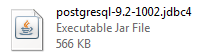
\includegraphics[scale=.5]{img/postgresql-file.png}
	\end{center}

	Ya finalmente podemos ejecutar el proyecto, la salida por pantalla sería la siguiente: 
	
	\begin{lstlisting}
	coche_id: 3
	nombre:  mondeo

	coche_id: 4
	nombre:  jumpy
	\end{lstlisting}
\end{frame}

\section{Configurar schema.xml}
	\begin{frame}
		\frametitle{La estructura de schema.xml}
		\setbeamercovered{invisible}
		
		\begin{center}
			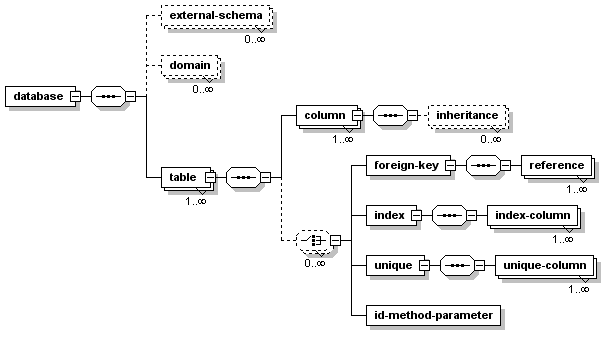
\includegraphics[scale=.4]{img/xml-config.png}
		\end{center}
	
		El esquema de base de datos de torque describe los elementos y atributos de la propia base de datos que estemos 			utillizando. A continuación se describe los principales elementos y las bases de datos compatibles actualmente.
	\end{frame}	
	
	\subsection{Elemento database}
		\begin{frame}[allowframebreaks]
			\frametitle{El elemento database}
			\setbeamercovered{invisible}
			
			Puede contener los siguientes 8 atributos:

			name: el nombre de la base de datos.
			defaultIdMethod: este se aplica a aquellas tablas que no tienen un atributo id definido. Por defecto es “none”. 			Normalmente se utiliza si no quieres ID’s generados.
			defaultJavaType: tipo predeterminado de las columnas de la base de datos ( “object” o “primitive”, por defecto es primitive).
			package: paquete base donde se generará los modelos de objetos asociados con la base de datos. Este reemplaza la propiedad “targetPackage” del archivo build.properties de Torque.
			baseClass: la clase base que se utilizará al generar el modelo de objetos.
			basePeer: la clase peer a utilizar al generar los pares del modelo de objetos.
			defaultJavaNamingMethod: este atributo determina como se convierten los nombres de las tablas y columnas en una clase Java o el nombre del método. Puede tener 3 valores diferentes:
			nochange: no se realizan cambios.
			underscore: se elimina el subrayado, la primera letra y después de un guión se pone la letra en mayúscula, el resto de caracteres en minúscula.
			javaname: con guiones bajos, pero las letras no se convierten en minúscula.
			heavyIndexing: agrega indices adicionales para columnas con varias claves primarias.
		\end{frame}

		\begin{frame}
			\frametitle{External-schema}
			\setbeamercovered{invisible}
			
			Incluye otro archivo de esquema. Puede haber 0 o más elementos de este tipo.

<Externa del esquema
           		filename = "extext-schema.xml" />
		\end{frame}
		
		\begin{frame}
			\frametitle{Domain}
			\setbeamercovered{invisible}
			
			Se utiliza para definir los atributos de las columnas.Puede haber 0 o más elementos de este tipo. 

<domain
           name="amount"
           type="NUMERIC"
           size="10"
           scale="2"
           default="0"
           description="amount domain" />
		\end{frame}

			\begin{frame}[fragile, allowframebreaks]
				\frametitle{Table}
				\setbeamercovered{invisible}
				
				Define las tablas y sus atributos:

\begin{lstlisting}[language=XML]
<table
	name="MY_TABLE"
	javaName="table"
	idMethod="idbroker"
	skipSql="false"
	baseClass="com.myapp.om.table.BaseClass"
	basePeer="com.myapp.om.table.BasePeer"
	javaNamingMethod="underscore"
	description="Table for Torque tests">

	<!-- column information here -->

</table>
\end{lstlisting}

El elemento table tiene los siguientes atributos asociados.

name: el nombre de la tabla que está siendo referenciada.
javaName: como se llamará esta tabla en Java.
idMethod: como s e crearán las claves primarias. Por defecto es nulo.
skipSql: valor booleano (true o false) que indica si hacer o no la generación de SQL para esta referencia.
abstract: valor booleano para generar la clase como abstracta o no.
baseClass: usado para la generación de OM Peer
basePeer: usado para la generación de OM Peer.
alias: define un alias para la tabla.
interface: especifica una interfaz que debería ser referenciada en la sección “implements” de la clase generada.
javaNamingMethod: especifica el nombre de la clase Java del correspondiente objeto OM. Este atributo reemplaza al atributo “defaultJavaNamingMehtod” del elemento de la base de datos (database).
description: se utiliza para la generación de documentación.

El elemento “table” también puede contener los siguientes elementos:
			\end{frame}
			
			\begin{frame}[fragile, allowframebreaks]
				\frametitle{column}
				\setbeamercovered{invisible}
				
				Puede haber 1 o más elementos de este tipo por tabla.

\begin{lstlisting}
<column
           		name="MY_COLUMN"
           		javaName="Column"
           		primaryKey="true"
           		required="true"
           		size="4"
           		type="VARCHAR"
           		javaNamingMethod="underscore">

           		<!-- inheritance info if necessary -->
</column>
\end{lstlisting}

Contiene los siguientes atributos:
name: nombre de la columna que está siendo referenciada.
javaName: como se llamará esta columna en Java.
primaryKey: valor booleano que indica si es la clave primaria o no. (true o false)
required: indica si el valor es requerido.(true o false, por defecto es false)
type: de que tipo es la columna.
javaType: el tipo de la columna en Java.
size: cuantos carácteres o digitos van a ser almacenados.
default: valor por defecto si al insertar está vacio.
autoIncrement: si este campo tiene autoincremento no. (true o false, por defecto es false)
inheritance. Indica si tiene herencia. Puede tomar los valores “single” o “false”.

javaNamingMethod: especifica el nombre que será utilizado en la clase Java del correspondiente objeto OM. Este atributo reemplaza al atributo “defaultJavaNamingMehtod” del elemento de la base de datos (database).

description: se utiliza para la generación de documentación.

			\end{frame}			
			
			\begin{frame}[fragile, allowframebreaks]
				\frametitle{Foreing-key}
				\setbeamercovered{invisible}
				
				Puede haber 0 o más elementos de este tipo por tabla.

\begin{lstlisting}
<foreign-key foreignTable="MY_TABLE"
	name="MY_TABLE_FK"
	onUpdate="none"
	onDelete="none">
	
	<!-- reference info -->
	<reference
	local="[columna_local]"
	foreign="[columna_foreign]"/>
</foreign-key>
\end{lstlisting}

Este elemento tiene 4 atributos:
foreignTable: el nombre de la tabla donde se encuentra la clave foránea.
name: el nombre de la clave foránea.
onUpdate: acción a realizar cuando se actualiza el valor en foreignTable.
onDelete: acción a realizar cuando se elimina el valor en foreingTable.
			\end{frame}
			
			\begin{frame}[fragile, allowframebreaks]
				\frametitle{Index e index-column}
				\setbeamercovered{invisible}
				
				Puede haber 0 o más elementos de este tipo por tabla.

\begin{lstlisting}
<index name="MY_INDEX">
	<!-- index-column info -->
</index>
\end{lstlisting}

El elemento index tiene 1 atributo asociado:
name: el nombre del índice. 
Puede contener 1 o más elementos  del tipo:

\begin{lstlisting}
<index-column name="INDEX_COLUMN"/>
\end{lstlisting}

Tiene solo un atributo: “name” que indica el nombre del índice de la columna. Este elemento no puede contener otros elementos.
			\end{frame}	
			
\section{Uso de Torque}
	\subsection{Las clases generadas}
	\subsection{Insertar filas}
	\subsection{La clase estática}
	\subsection{Seleccionar filas}
	\subsection{Actualizar filas}
	\subsection{Eliminar filas}
	
\section{Aplicación de ejemplo}

\end{document}